% Options for packages loaded elsewhere
\PassOptionsToPackage{unicode}{hyperref}
\PassOptionsToPackage{hyphens}{url}
%
\documentclass[
  ignorenonframetext,
]{beamer}
\usepackage{pgfpages}
\setbeamertemplate{caption}[numbered]
\setbeamertemplate{caption label separator}{: }
\setbeamercolor{caption name}{fg=normal text.fg}
\beamertemplatenavigationsymbolsempty
% Prevent slide breaks in the middle of a paragraph
\widowpenalties 1 10000
\raggedbottom
\setbeamertemplate{part page}{
  \centering
  \begin{beamercolorbox}[sep=16pt,center]{part title}
    \usebeamerfont{part title}\insertpart\par
  \end{beamercolorbox}
}
\setbeamertemplate{section page}{
  \centering
  \begin{beamercolorbox}[sep=12pt,center]{part title}
    \usebeamerfont{section title}\insertsection\par
  \end{beamercolorbox}
}
\setbeamertemplate{subsection page}{
  \centering
  \begin{beamercolorbox}[sep=8pt,center]{part title}
    \usebeamerfont{subsection title}\insertsubsection\par
  \end{beamercolorbox}
}
\AtBeginPart{
  \frame{\partpage}
}
\AtBeginSection{
  \ifbibliography
  \else
    \frame{\sectionpage}
  \fi
}
\AtBeginSubsection{
  \frame{\subsectionpage}
}

\usepackage{amsmath,amssymb}
\usepackage{iftex}
\ifPDFTeX
  \usepackage[T1]{fontenc}
  \usepackage[utf8]{inputenc}
  \usepackage{textcomp} % provide euro and other symbols
\else % if luatex or xetex
  \usepackage{unicode-math}
  \defaultfontfeatures{Scale=MatchLowercase}
  \defaultfontfeatures[\rmfamily]{Ligatures=TeX,Scale=1}
\fi
\usepackage{lmodern}
\ifPDFTeX\else  
    % xetex/luatex font selection
\fi
% Use upquote if available, for straight quotes in verbatim environments
\IfFileExists{upquote.sty}{\usepackage{upquote}}{}
\IfFileExists{microtype.sty}{% use microtype if available
  \usepackage[]{microtype}
  \UseMicrotypeSet[protrusion]{basicmath} % disable protrusion for tt fonts
}{}
\makeatletter
\@ifundefined{KOMAClassName}{% if non-KOMA class
  \IfFileExists{parskip.sty}{%
    \usepackage{parskip}
  }{% else
    \setlength{\parindent}{0pt}
    \setlength{\parskip}{6pt plus 2pt minus 1pt}}
}{% if KOMA class
  \KOMAoptions{parskip=half}}
\makeatother
\usepackage{xcolor}
\newif\ifbibliography
\setlength{\emergencystretch}{3em} % prevent overfull lines
\setcounter{secnumdepth}{-\maxdimen} % remove section numbering


\providecommand{\tightlist}{%
  \setlength{\itemsep}{0pt}\setlength{\parskip}{0pt}}\usepackage{longtable,booktabs,array}
\usepackage{calc} % for calculating minipage widths
\usepackage{caption}
% Make caption package work with longtable
\makeatletter
\def\fnum@table{\tablename~\thetable}
\makeatother
\usepackage{graphicx}
\makeatletter
\def\maxwidth{\ifdim\Gin@nat@width>\linewidth\linewidth\else\Gin@nat@width\fi}
\def\maxheight{\ifdim\Gin@nat@height>\textheight\textheight\else\Gin@nat@height\fi}
\makeatother
% Scale images if necessary, so that they will not overflow the page
% margins by default, and it is still possible to overwrite the defaults
% using explicit options in \includegraphics[width, height, ...]{}
\setkeys{Gin}{width=\maxwidth,height=\maxheight,keepaspectratio}
% Set default figure placement to htbp
\makeatletter
\def\fps@figure{htbp}
\makeatother

\makeatletter
\@ifpackageloaded{caption}{}{\usepackage{caption}}
\AtBeginDocument{%
\ifdefined\contentsname
  \renewcommand*\contentsname{Table of contents}
\else
  \newcommand\contentsname{Table of contents}
\fi
\ifdefined\listfigurename
  \renewcommand*\listfigurename{List of Figures}
\else
  \newcommand\listfigurename{List of Figures}
\fi
\ifdefined\listtablename
  \renewcommand*\listtablename{List of Tables}
\else
  \newcommand\listtablename{List of Tables}
\fi
\ifdefined\figurename
  \renewcommand*\figurename{Figure}
\else
  \newcommand\figurename{Figure}
\fi
\ifdefined\tablename
  \renewcommand*\tablename{Table}
\else
  \newcommand\tablename{Table}
\fi
}
\@ifpackageloaded{float}{}{\usepackage{float}}
\floatstyle{ruled}
\@ifundefined{c@chapter}{\newfloat{codelisting}{h}{lop}}{\newfloat{codelisting}{h}{lop}[chapter]}
\floatname{codelisting}{Listing}
\newcommand*\listoflistings{\listof{codelisting}{List of Listings}}
\makeatother
\makeatletter
\makeatother
\makeatletter
\@ifpackageloaded{caption}{}{\usepackage{caption}}
\@ifpackageloaded{subcaption}{}{\usepackage{subcaption}}
\makeatother
\ifLuaTeX
  \usepackage{selnolig}  % disable illegal ligatures
\fi
\usepackage{bookmark}

\IfFileExists{xurl.sty}{\usepackage{xurl}}{} % add URL line breaks if available
\urlstyle{same} % disable monospaced font for URLs
\hypersetup{
  pdftitle={Predicting Student Performance},
  pdfauthor={Daniel Posmik, Jizhou Tian, Aristofanis Rontogiannis},
  hidelinks,
  pdfcreator={LaTeX via pandoc}}

\title{Predicting Student Performance}
\subtitle{Linear Models (PHP2601), Prof.~Ani Eloyan}
\author{Daniel Posmik, Jizhou Tian, Aristofanis Rontogiannis}
\date{2024-12-10}

\begin{document}
\frame{\titlepage}

\renewcommand*\contentsname{Table of contents}
\begin{frame}[allowframebreaks]
  \frametitle{Table of contents}
  \tableofcontents[hideallsubsections]
\end{frame}
\begin{frame}[fragile]{EDA and the Linear Model}
\phantomsection\label{eda-and-the-linear-model}
\begin{block}{Introduction}
\phantomsection\label{introduction}
We will be analyzing educational data to understand the predictors of
student performance. Specifically, we seek to \textbf{understand whether
five predictors -- as a subset of an exhaustive list of potential
predictors -- are significant predictors of student performance}.

Testing the significant of a subset of predictors is becoming
increasingly important in modern statistical questions, especially with
more information becoming available.

We will be using a publicly available dataset from Kaggle that contains
information about students and their exam scores.
\end{block}

\begin{block}{Hypothesis to be Tested}
\phantomsection\label{hypothesis-to-be-tested}
We are interested in:

\begin{itemize}
\tightlist
\item
  Hours Studied
\item
  Attendance
\item
  Sleep Hours
\item
  Previous Scores
\item
  Tutoring Sessions
\end{itemize}

We can formalize this question as follows:

\begin{itemize}
\tightlist
\item
  \(H_0: \begin{bmatrix} 1_{[0, \cdots, p+1]}, & 0_{[p+2, \cdots, P]} \end{bmatrix} \cdot \begin{bmatrix} \beta_0 & \cdots & \beta_{P} \end{bmatrix}^T = \beta_0 + \cdots + \beta_{p+1} = 0\)
\item
  \(H_A: \{\beta_1 \neq 0\} \cap \cdots \cap \{\beta_5 \neq 0\}\)
\end{itemize}

Observe the 0-indexed variables from \(p+2\) to \(P\).
\end{block}

\begin{block}{Exploratory Data Analysis (EDA)}
\phantomsection\label{exploratory-data-analysis-eda}
\begin{figure}[H]

{\centering 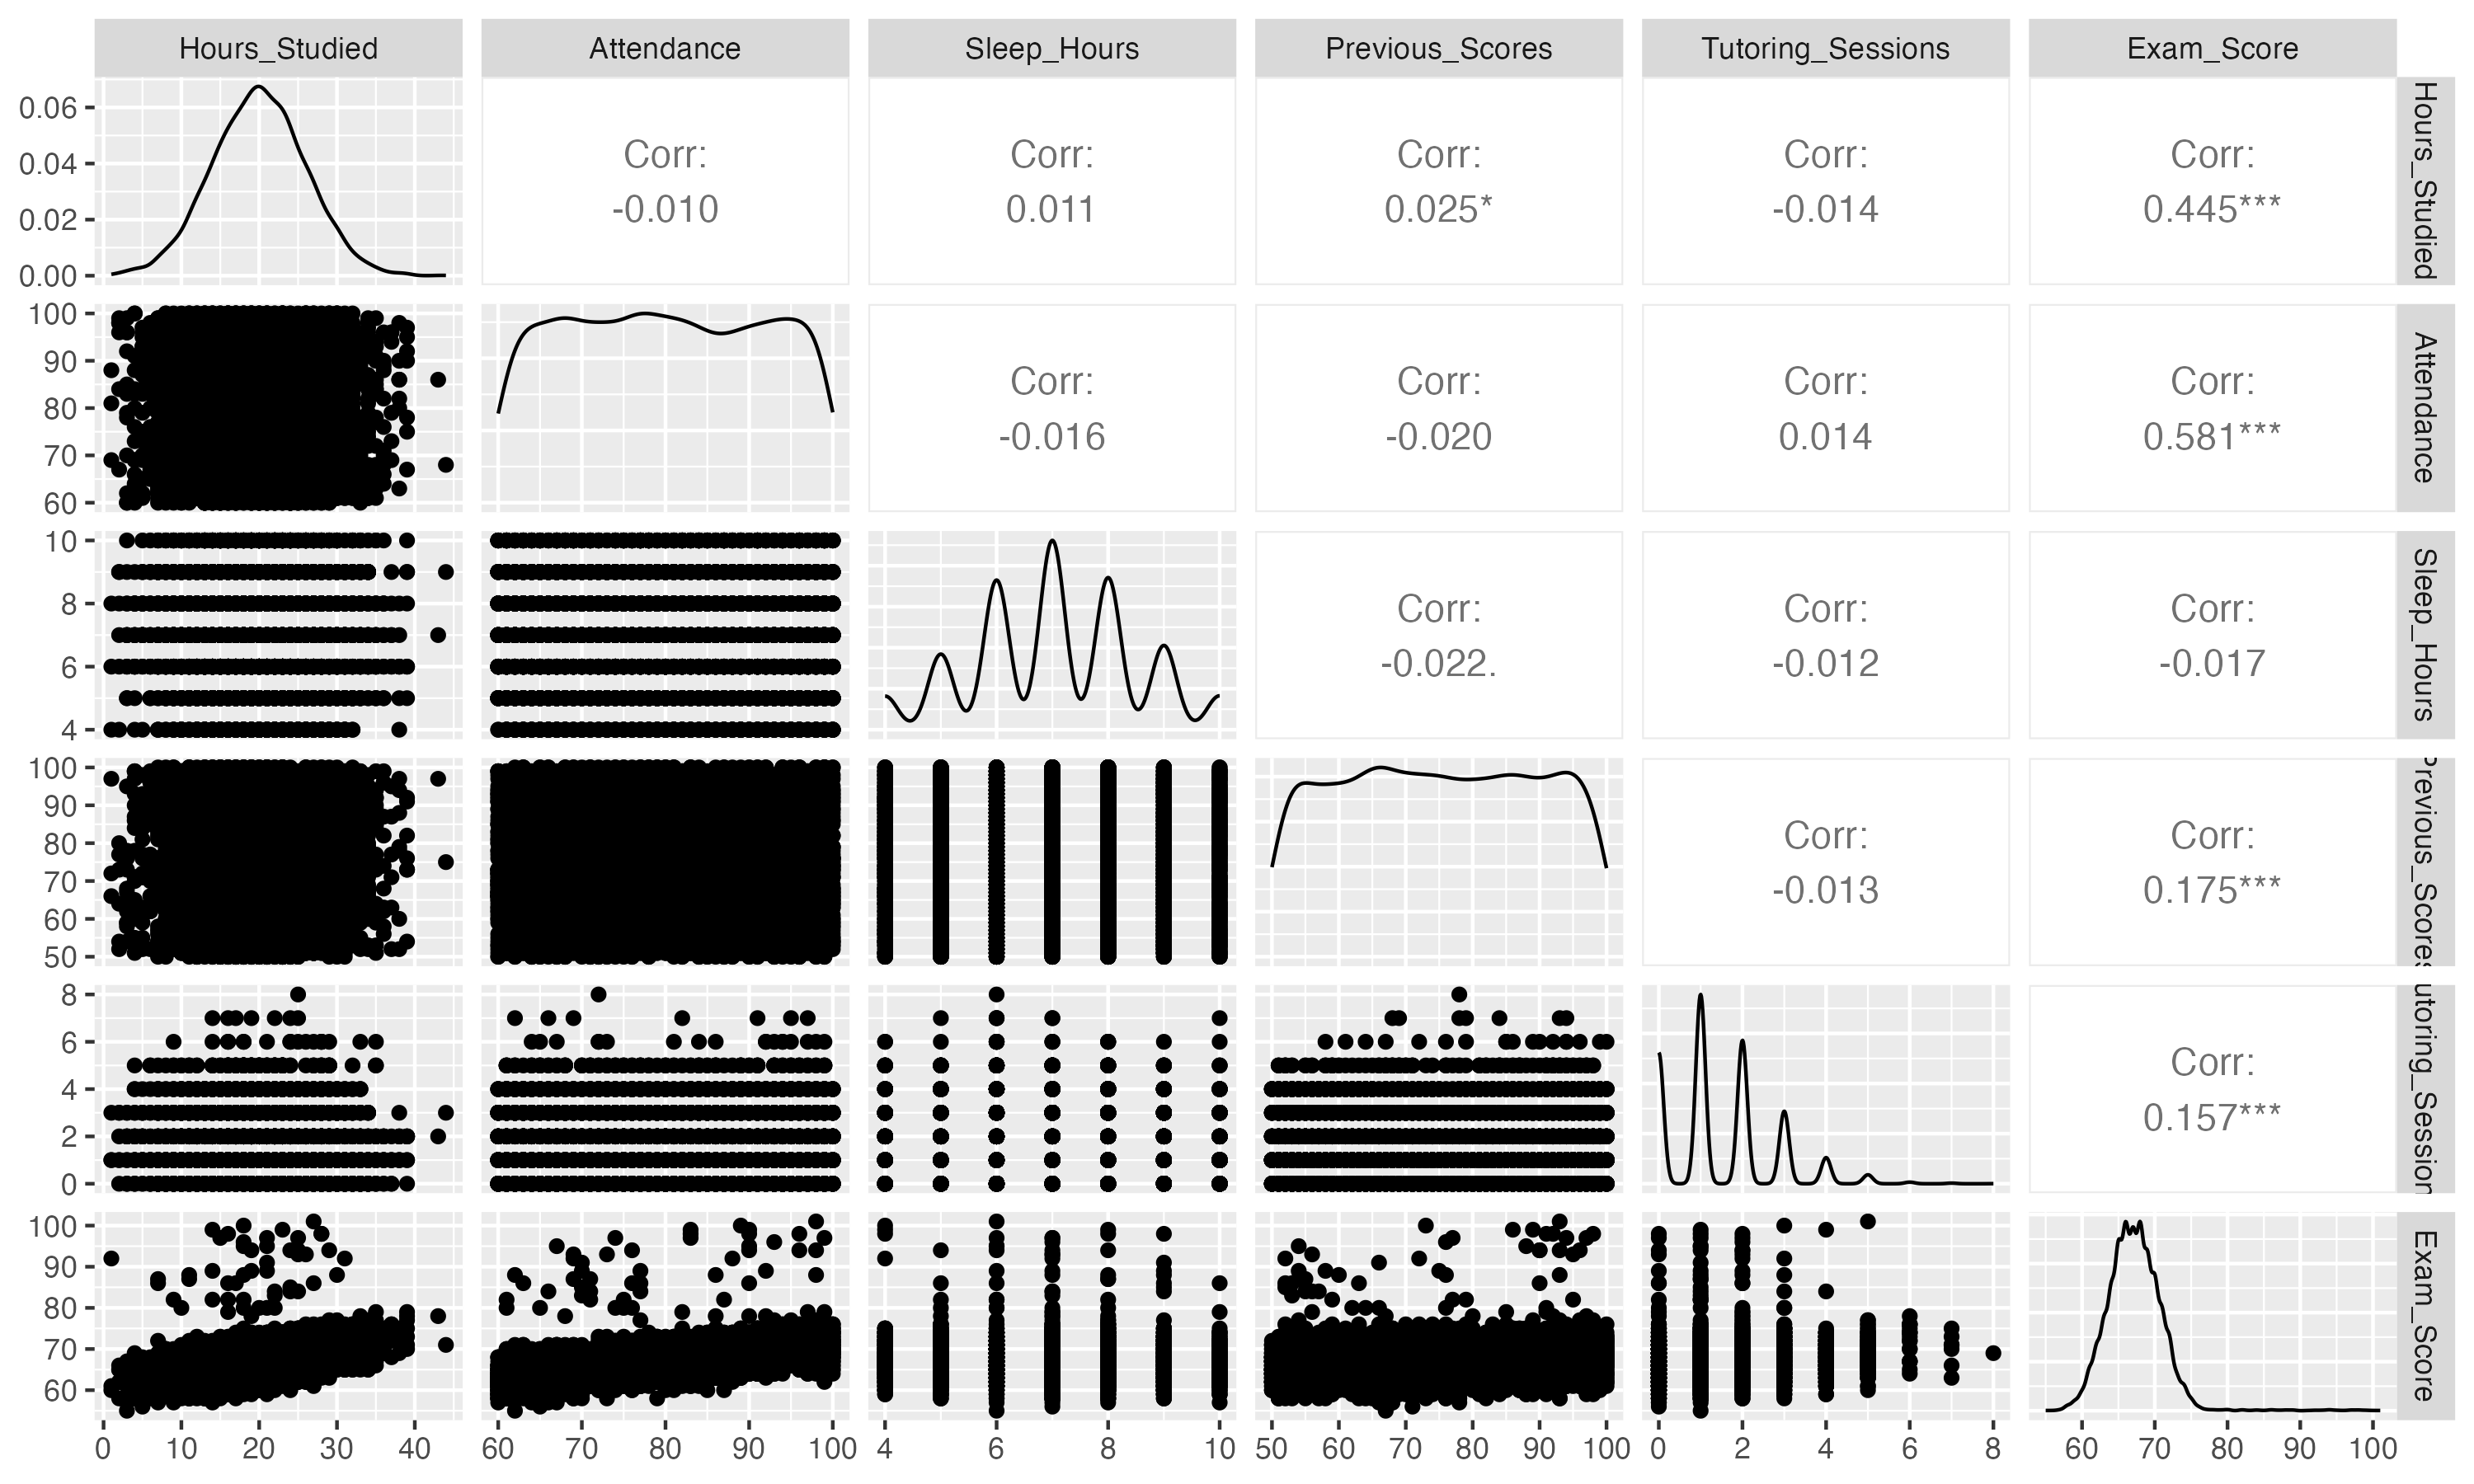
\includegraphics{correlation_matrix.png}

}

\caption{Correlation Matrix}

\end{figure}%
\end{block}

\begin{block}{Variable Transformations}
\phantomsection\label{variable-transformations}
We will transform the variables to ensure that the assumptions of the
linear model are met.

\begin{figure}[H]

{\centering 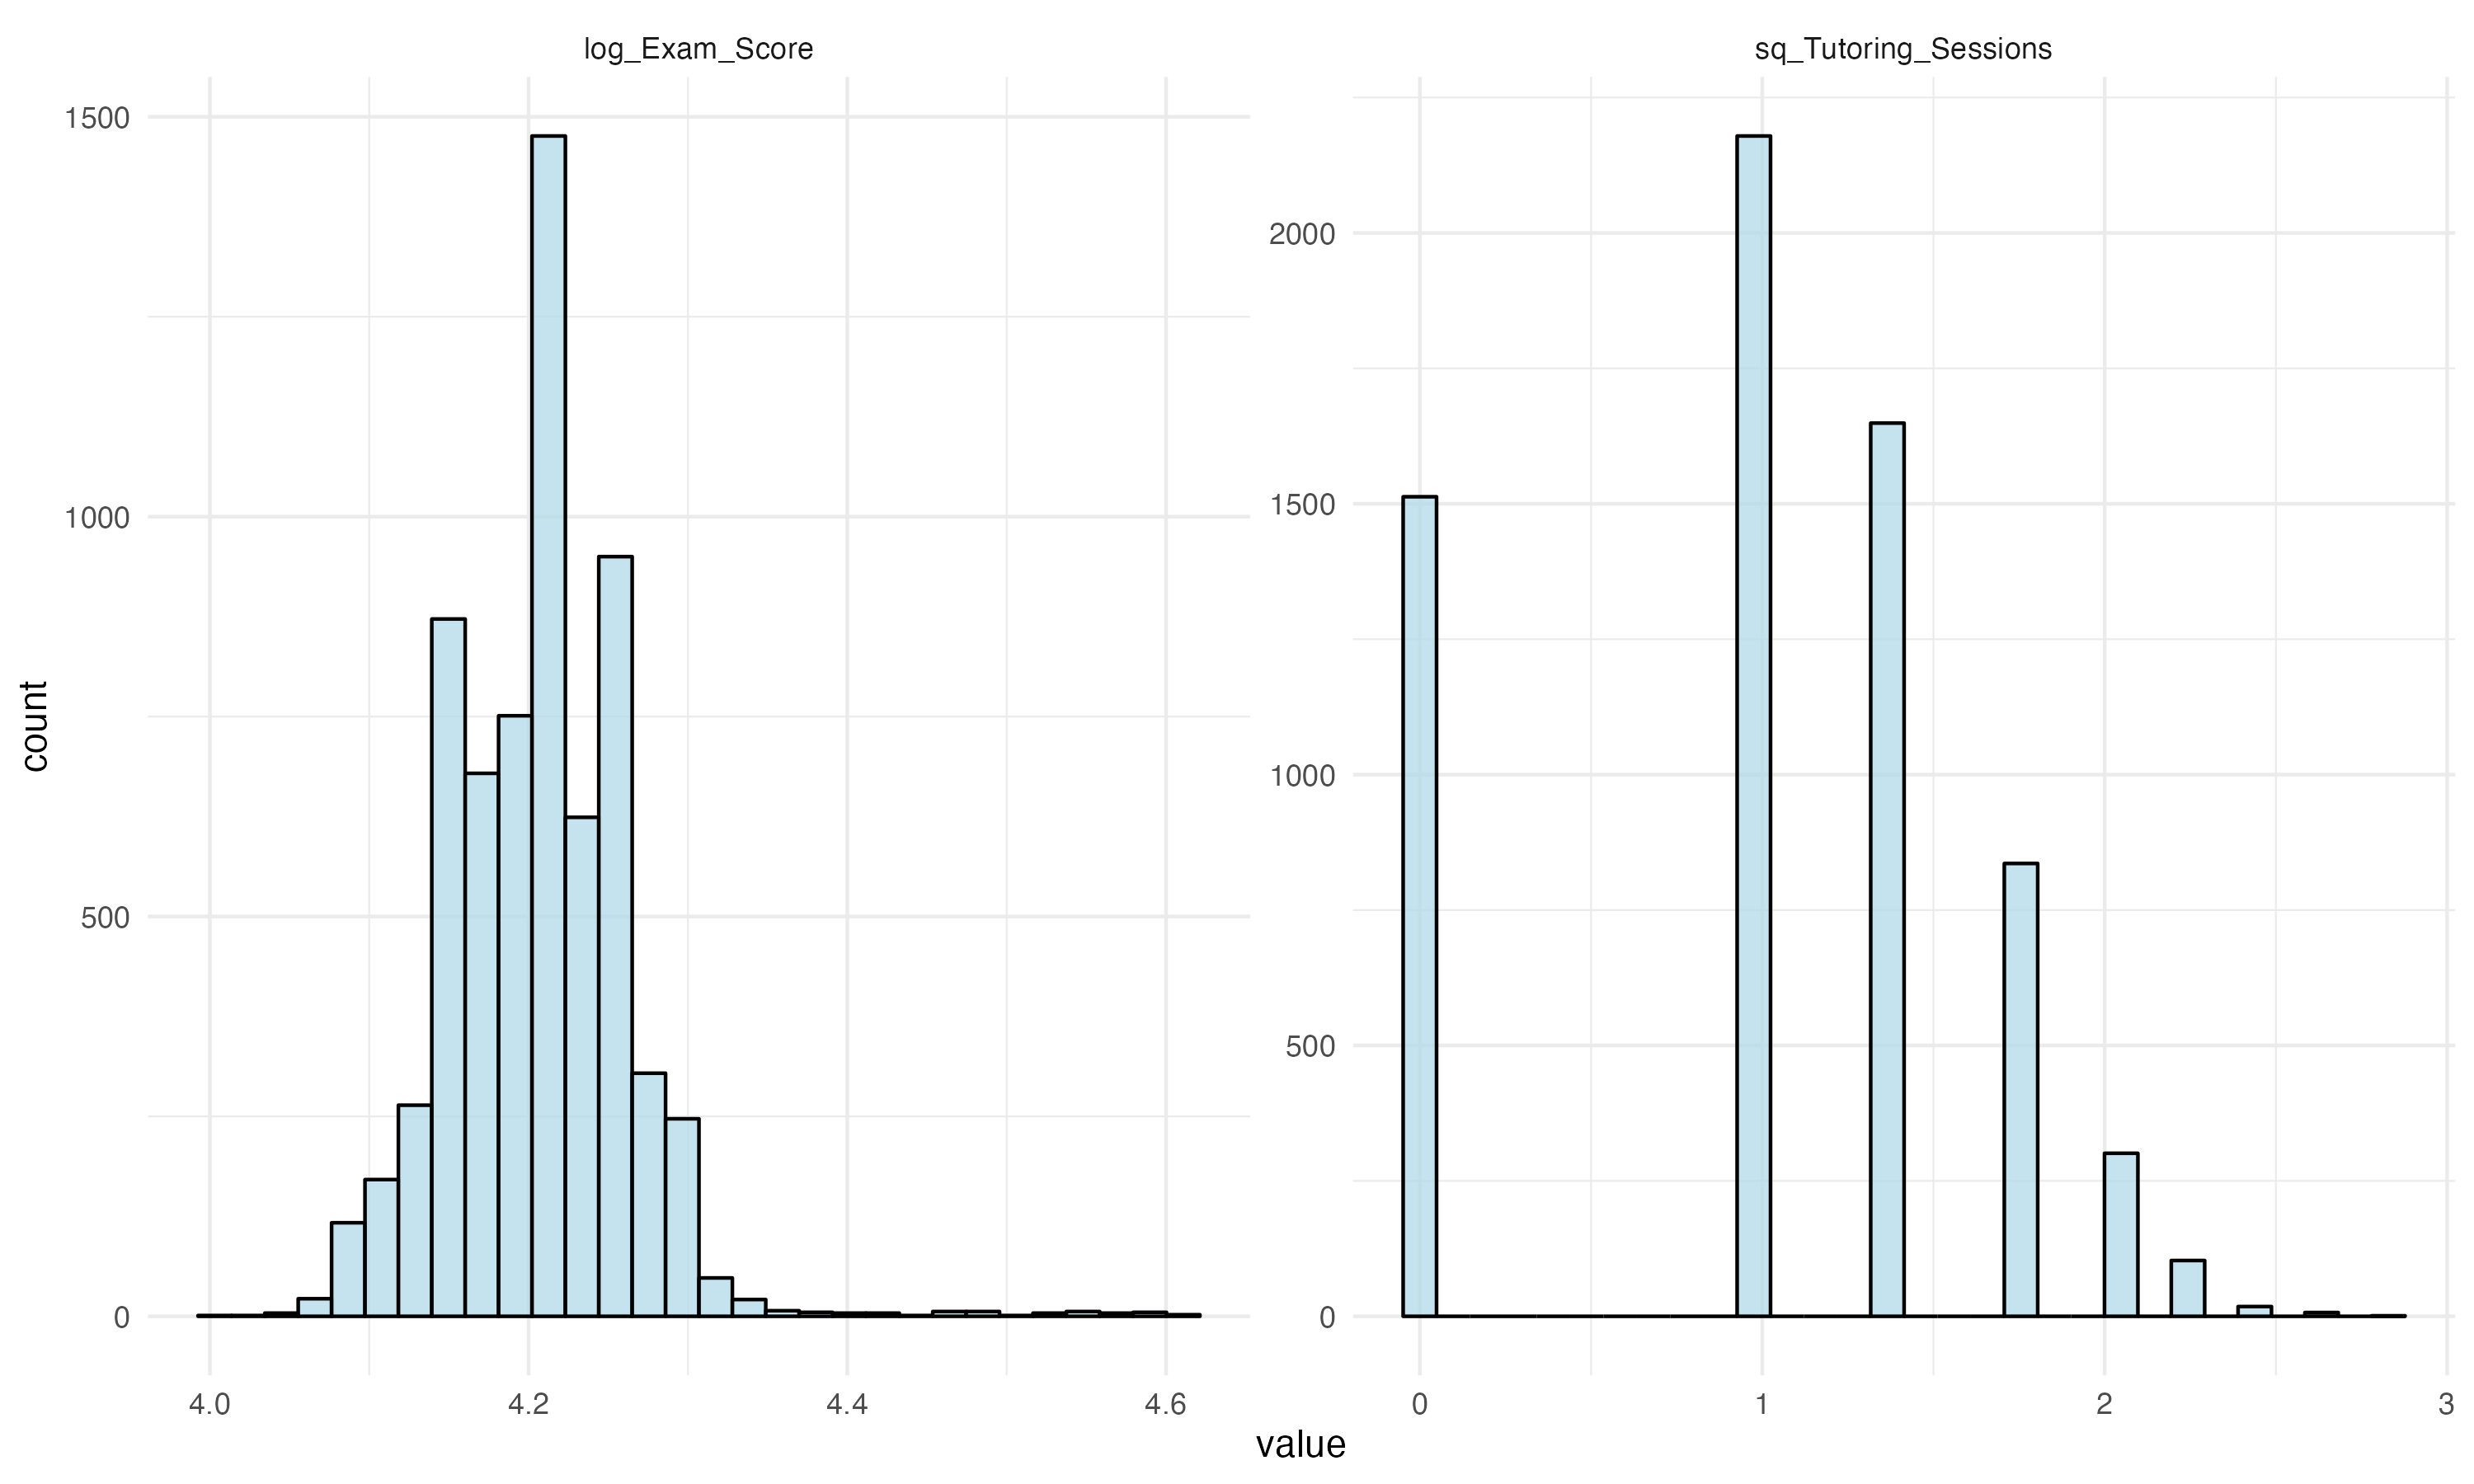
\includegraphics{histograms.png}

}

\caption{Variable Transformation}

\end{figure}%

We use log and square root transformations to ensure that the residuals
are normally distributed.
\end{block}

\begin{block}{The Linear Model}
\phantomsection\label{the-linear-model}
Let us begin by discussing the assumptions of linear regression model.
In a Gauss-Markov setting, we assume that our linear model is of the
form:

\[
Y = \begin{bmatrix} Y_1 \\ Y_2 \\ \vdots \\ Y_n \end{bmatrix} = 
\begin{bmatrix}
1 & X_{12} & X_{13} & \cdots & X_{1(p+1)} \\
1 & X_{22} & X_{23} & \cdots & X_{2(p+1)} \\
\vdots & \vdots & \vdots & \ddots & \vdots \\
1 & X_{n2} & X_{n3} & \cdots & X_{n(p+1)}
\end{bmatrix} 
\begin{bmatrix} \beta_0 \\ \beta_1 \\ \beta_2 \\ \vdots \\ \beta_p \end{bmatrix} + 
\begin{bmatrix} \epsilon_1 \\ \epsilon_2 \\ \vdots \\ \epsilon_n \end{bmatrix}
\]

where \(\mathbb{E}[\epsilon] = 0\) and
\(\text{Var}[\epsilon] = \sigma^2I\) denote the zero-mean and constant
variance assumptions. In our case, we begin with \(p = 5\), i.e.~our
design matrix has \(p+1\) columns, accounting for the intercept term.
\end{block}

\begin{block}{Solving for \(\hat{\beta}\)}
\phantomsection\label{solving-for-hatbeta}
We can solve for \(\hat{\beta}\) via the normal equations:

\[
\begin{aligned}
\hat{\beta} = &(X^TX)^{g}X^TY \\
= &\left( 
\begin{bmatrix} 1 & 1 & \cdots & 1 \\ X_{12} & X_{22} & \cdots & X_{n2} \\ \vdots & \vdots & \ddots & \vdots \\ X_{1(p+1)} & X_{2(p+1)} & \cdots & X_{n(p+1)} \end{bmatrix} 
\begin{bmatrix} 1 & X_{12} & \cdots & X_{1(p+1)} \\ 1 & X_{22} & \cdots & X_{2(p+1)} \\ \vdots & \vdots & \ddots & \vdots \\ 1 & X_{n2} & \cdots & X_{n(p+1)} \end{bmatrix} 
\right)^{g} 
\cdot \\
&\begin{bmatrix} 1 & 1 & \cdots & 1 \\ X_{12} & X_{22} & \cdots & X_{n2} \\ \vdots & \vdots & \ddots & \vdots \\ X_{1(p+1)} & X_{2(p+1)} & \cdots & X_{n(p+1)} \end{bmatrix} 
\begin{bmatrix} Y_1 \\ Y_2 \\ \vdots \\ Y_n \end{bmatrix}
\end{aligned}
\]

In our case, all predictors but Sleep Hours are significant predictors
of exam scores, even at a 1\% level of significance.
\end{block}

\begin{block}{Estimability of the Hypothesis}
\phantomsection\label{estimability-of-the-hypothesis}
Question: \textbf{Can we estimate an object \(K^T \beta\) with our data
\(X\)?}

Formally, we say that if \(\exists ~ A ~ \text{s.t. } X^TA = K^T\),
i.e.~\(K^T\) can be expressed as a linear combination of \(X\) and some
matrix \(A\), then \(K^T \beta\) is estimable.

In our case, this is straightforward to verify. Can we think of an
example when this is not true? (Hint: Dimension ``mismatch'')
\end{block}

\begin{block}{Distribution of \(K^T \beta\)}
\phantomsection\label{distribution-of-kt-beta}
Since \(K^T \beta\) estimable, its best linear unbiased estimator (BLUE)
is given by:

\[
\begin{aligned}
\mathbf{K_i}^T \hat{\beta} &\sim \textit{N}(\mathbf{K_i}^T (X^T X)^g X^T X \beta, \sigma^2 \mathbf{K_i}^T(X^TX)^{g}\mathbf{K_i}) \quad \text{and} \\ 
\mathbf{K}^T \hat{\beta} &\sim \textit{N}(\mathbf{K}^T (X^T X)^g X^T X \beta, \sigma^2 \mathbf{K}^T(X^TX)^{g}\mathbf{K}) 
\end{aligned}
\]

This object \(K^T \beta\) may seem a bit arbitrary, even useless, at
first. However, it is in fact the building block for the test statistic
we will construct now!
\end{block}

\begin{block}{Quadratic Form in our Joint Testing Procedure}
\phantomsection\label{quadratic-form-in-our-joint-testing-procedure}
Suppose \(H := K (X^T X)^g K^T\), then

\[
\begin{aligned}
(K \beta)^T (\sigma^2 H)^{-1} (K \hat{\beta}) &\sim \chi^2_{\text{df} = \text{rank}(H)}(\lambda) \\
\end{aligned}
\]

where the non-centrality parameter
\(\lambda = \frac{1}{2} (K \beta)^T (\sigma^2 H)^{-1}(K \beta)\) is the
well-known distributional result of a normal quadratic form.

Finally, our F Statistic:

\[
\begin{aligned}
F := \frac{\left((K \beta)^T (\sigma^2 H)^{-1}(K \beta)\right) / \text{rank}(H)}{\text{RSS}/(n-p)}
\sim \frac{\chi^2 (\lambda)}{\chi^2} \sim F_{\text{rank}(H), n-p}(\lambda)
\end{aligned}
\]

We have successfully constructed a statistical test that allows us to
test our hypothesis with a simple F-test. In \texttt{R}, we can use the
\texttt{anova()} function to perform this test.
\end{block}

\begin{block}{Results}
\phantomsection\label{results}
\begin{figure}[H]

{\centering 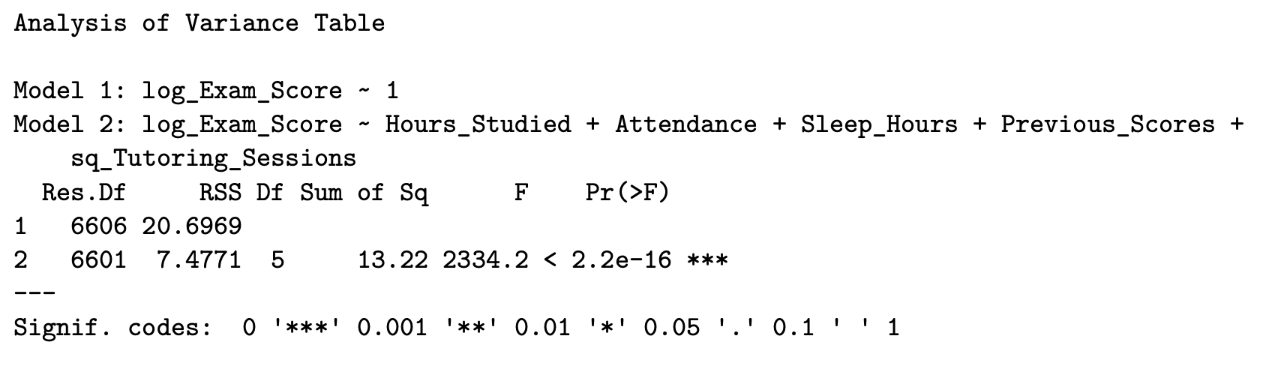
\includegraphics{anova-results.png}

}

\caption{F-Test Results}

\end{figure}%

The result shows that under the null hypothesis, the probability of
getting a more extreme result than our calculate F-test statistics
\(\text{Pr}(>F)\) is \(2.2e− 16\).

This evidence would lead us to reject the null hypothesis and conclude
that our subset of predictors is indeed a significant predictor of exam
scores
\end{block}
\end{frame}

\begin{frame}{Elastic Net}
\phantomsection\label{elastic-net}
\end{frame}

\begin{frame}{Why Use Elastic Net?}
\phantomsection\label{why-use-elastic-net}
\begin{itemize}
\tightlist
\item
  \textbf{Limitations of Lasso}: May select only one variable from a
  group of highly correlated predictors.
\item
  \textbf{Limitations of Ridge}: Cannot produce sparse models (i.e., no
  feature selection).
\item
  \textbf{Elastic Net Advantage}:

  \begin{itemize}
  \tightlist
  \item
    Encourages group selection.
  \item
    Balances sparsity and multicollinearity handling.
  \end{itemize}
\end{itemize}
\end{frame}

\begin{frame}{Elastic Net Formula}
\phantomsection\label{elastic-net-formula}
Elastic Net adds two penalty terms:

\[ \min_{\beta} \Bigg( \sum_{i=1}^n (y_i - X_i \beta)^2 + \lambda_1 \|\beta\|_1 + \lambda_2 \|\beta\|_2^2 \Bigg) \]

\begin{itemize}
\tightlist
\item
  \(\|\beta\|_1\): Lasso penalty (L1).
\item
  \(\|\beta\|_2^2\): Ridge penalty (L2).
\item
  \(\lambda_1, \lambda_2\): Regularization parameters.
\end{itemize}
\end{frame}

\begin{frame}{Tuning Parameters in Elastic Net}
\phantomsection\label{tuning-parameters-in-elastic-net}
\begin{enumerate}
\tightlist
\item
  \textbf{\(\alpha\)}: Controls the mix between Ridge and Lasso.

  \begin{itemize}
  \tightlist
  \item
    \(\alpha = 0\): Ridge.
  \item
    \(\alpha = 1\): Lasso.
  \item
    \(0 < \alpha < 1\): Elastic Net.
  \end{itemize}
\item
  \textbf{\(\lambda\)}: Controls the overall strength of regularization.
\end{enumerate}

\begin{block}{Grid Search:}
\phantomsection\label{grid-search}
\begin{itemize}
\tightlist
\item
  Perform cross-validation to find optimal values of \(\alpha\) and
  \(\lambda\).
\end{itemize}
\end{block}
\end{frame}

\begin{frame}{Elastic Net: Geometric Interpretation}
\phantomsection\label{elastic-net-geometric-interpretation}
\begin{itemize}
\tightlist
\item
  Elastic Net creates a penalty region combining L1 (diamond) and L2
  (circle).
\item
  Encourages sparsity while handling correlated features.
\end{itemize}

\begin{figure}[H]

{\centering 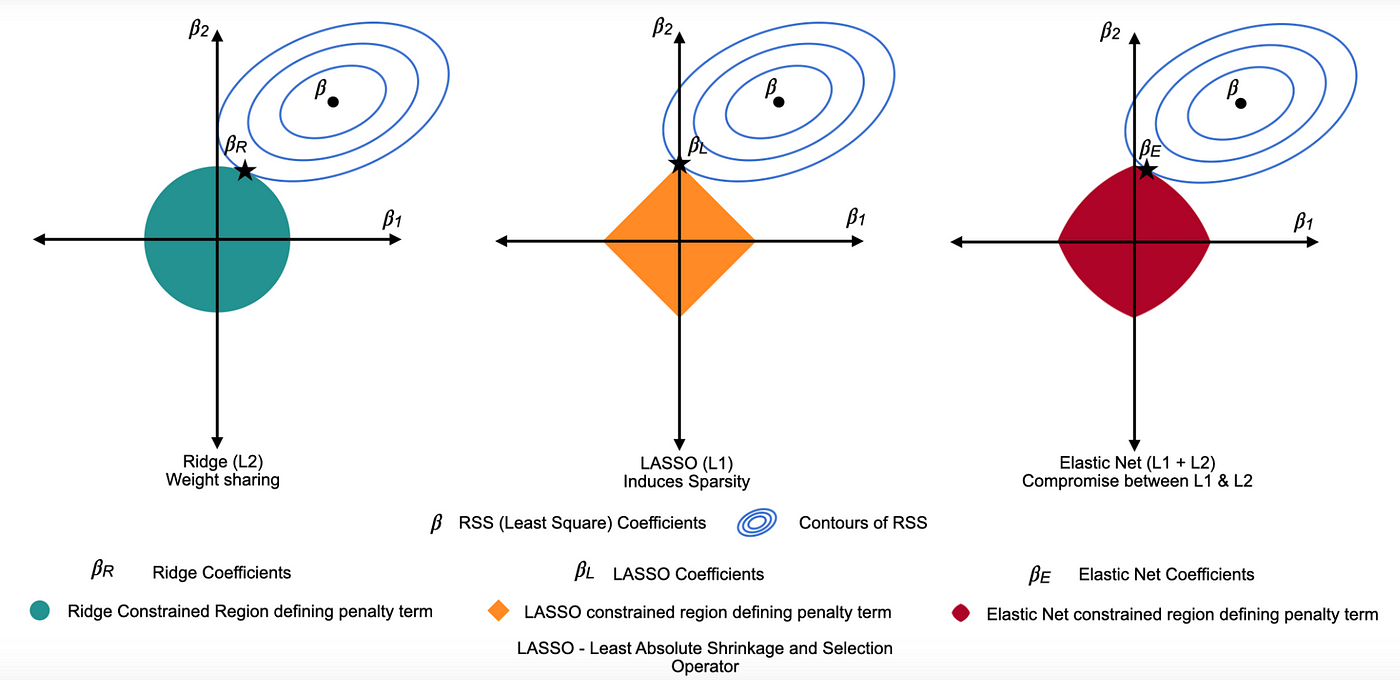
\includegraphics{visualization_Elastic.png}

}

\caption{Elastic Net compared to Lasso and Ridge Regression}

\end{figure}%
\end{frame}

\begin{frame}{Elastic Net with Continuous Outcome}
\phantomsection\label{elastic-net-with-continuous-outcome}
The \(R^2\) on the test data is calculated to be approximately \(76\%\),
meaning our model is able to explain \(76\%\) of the variance in Exam
Score in the test dataset

\begin{figure}[H]

{\centering 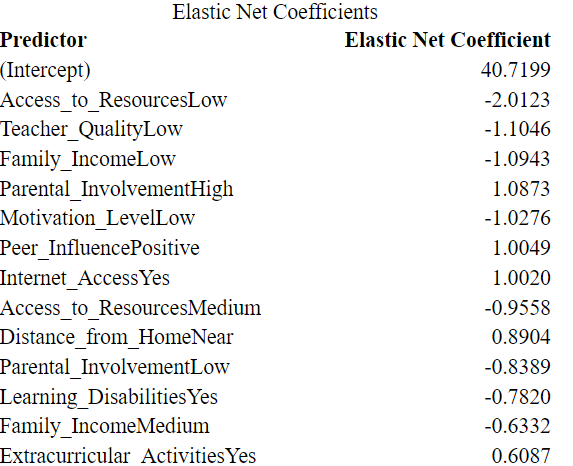
\includegraphics[width=0.4\textwidth,height=\textheight]{elastnettable1.png}

}

\caption{The first 14 rows of the Elastic Net coefficients table}

\end{figure}%

\textbf{Note:} Elastic Net (or Lasso) did not drop any variables as all
predictors contribute to reducing the loss function, even with
regularization applied.
\end{frame}

\begin{frame}{Elastic Net with Binary Outcome}
\phantomsection\label{elastic-net-with-binary-outcome}
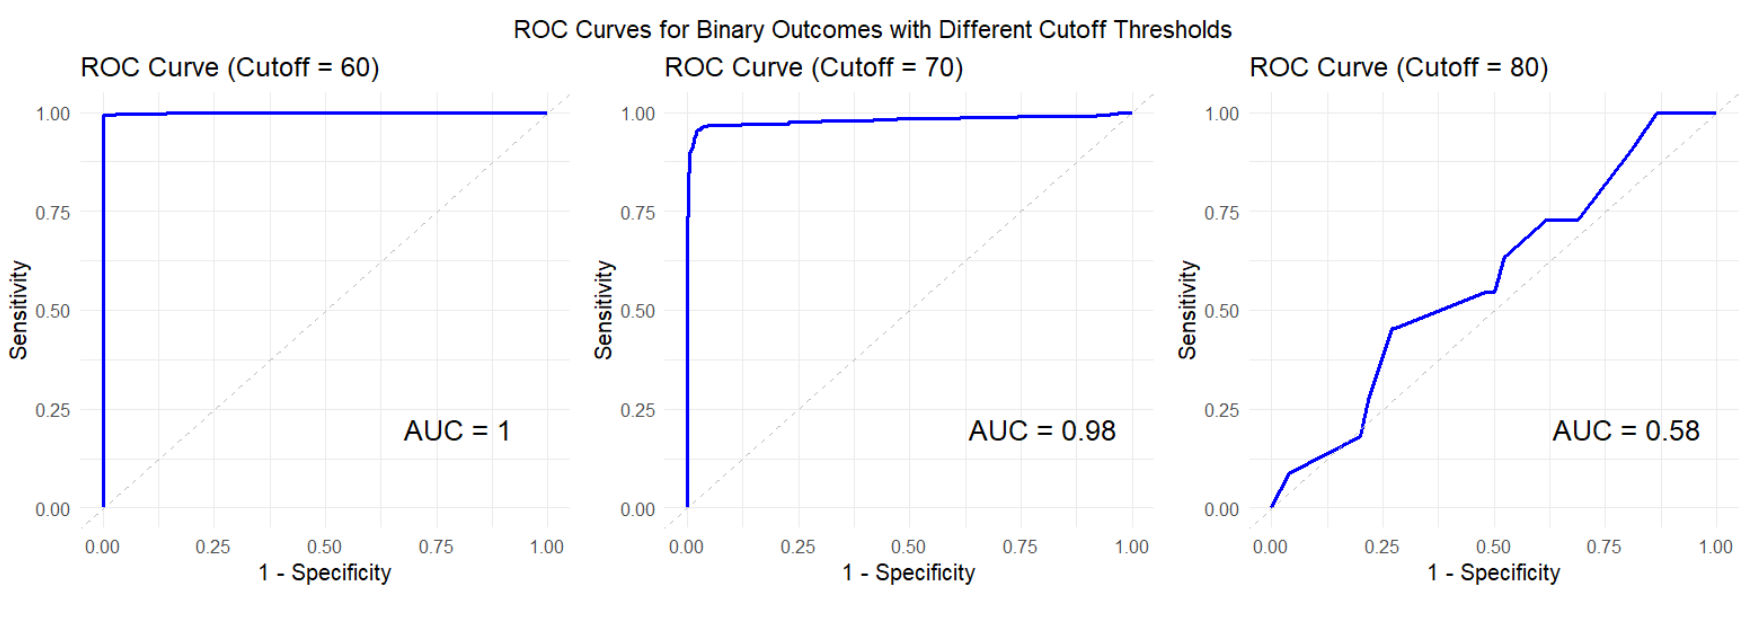
\includegraphics[width=1\textwidth,height=\textheight]{ROC_3plots.png}
\textbf{Note:} This is an imbalanced dataset as most of the students
have scored more than 60 in the exams. The median (and the mean) of the
dataset is very close to the 3rd quantile (69). For instance, if we use
threshold = 70, we can predict the probability a student's score is
within/out the top 25\% of the scores almost perfectly.
\end{frame}

\begin{frame}{Stochastic Gradient Boosting Machine (GBM) - Gradient
Boosting Machine Algorithm}
\phantomsection\label{stochastic-gradient-boosting-machine-gbm---gradient-boosting-machine-algorithm}
\end{frame}

\begin{frame}{What is Gradient Boosting?}
\phantomsection\label{what-is-gradient-boosting}
\begin{itemize}
\item
  \textbf{Definition}: Gradient boosting is a machine learning ensemble
  technique (ensemble models combine predictions from multiple base
  models to enhance overall performance) that sequentially combines the
  predictions of multiple weak learners, typically decision trees.
\item
  \textbf{Purpose}: It aims to improve overall predictive performance by
  optimizing the model's weights based on the errors of previous
  iterations, gradually reducing prediction errors and enhancing the
  model's accuracy.
\end{itemize}
\end{frame}

\begin{frame}{How It Works}
\phantomsection\label{how-it-works}
\begin{itemize}
\tightlist
\item
  \textbf{Step 1}: Start with a baseline model (e.g., mean prediction
  for regression)
\item
  \textbf{Step 2}: Compute residuals or errors from the current model
\item
  \textbf{Step 3}: Fit a new model to the residuals (weak learners like
  decision trees)
\item
  \textbf{Step 4}: Update the overall model by adding the new learner
\item
  \textbf{Step 5}: Repeat until convergence or a predefined number of
  iterations
\end{itemize}

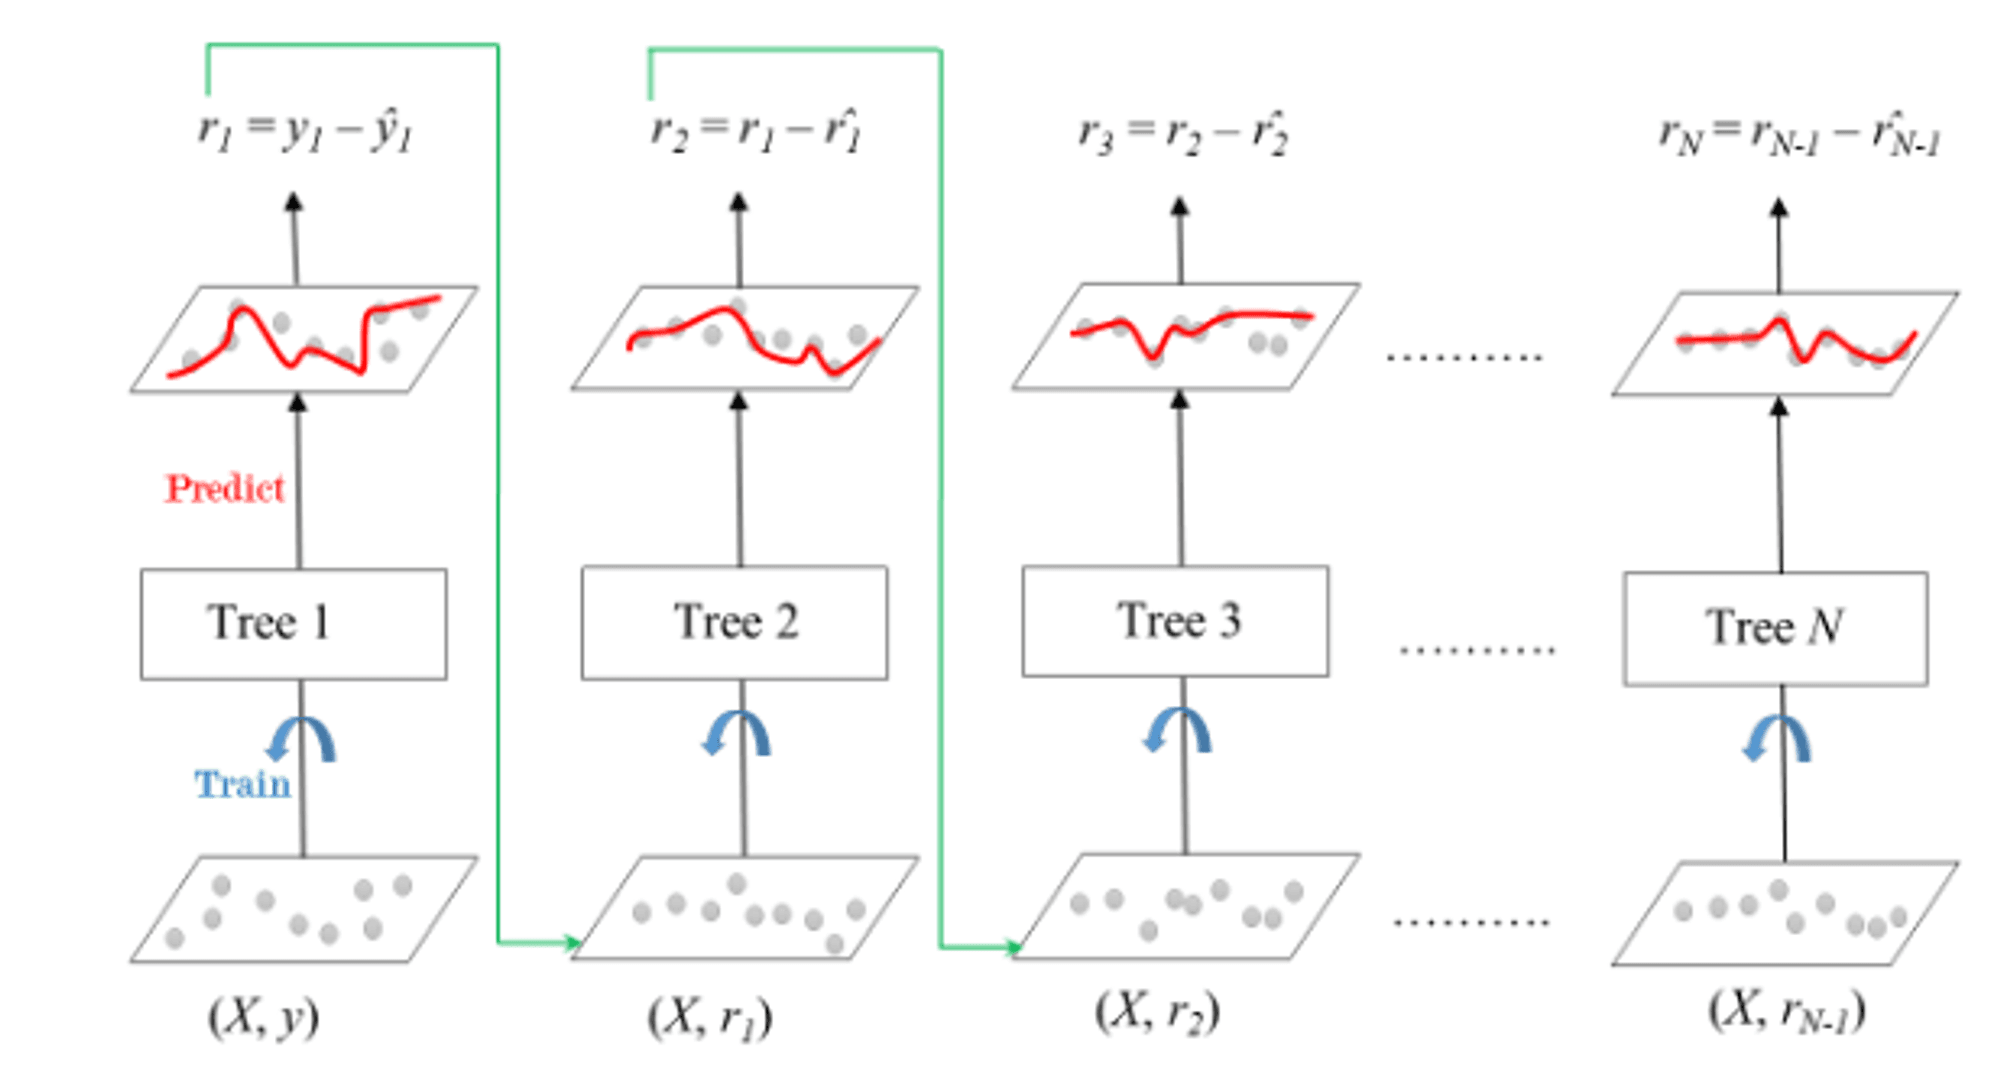
\includegraphics[width=0.75\textwidth,height=\textheight]{gbm_visual.png}
\end{frame}

\begin{frame}{In our dataset}
\phantomsection\label{in-our-dataset}
\begin{figure}[H]

{\centering 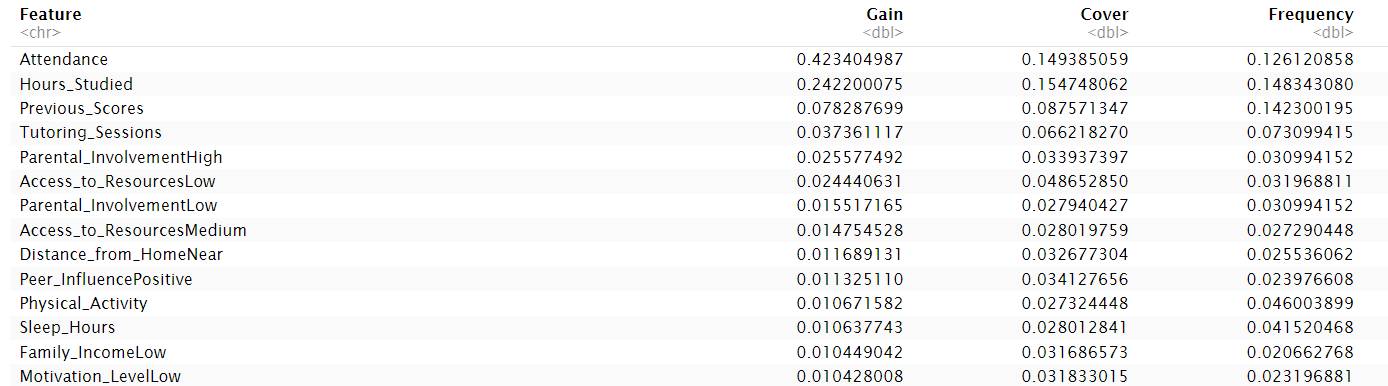
\includegraphics[width=0.8\textwidth,height=\textheight]{gbm_visual3.png}

}

\caption{Feature Importance Summary}

\end{figure}%

\begin{itemize}
\tightlist
\item
  \textbf{Feature}: Lists the features (variables) in the dataset.
\item
  \textbf{Gain}: Contribution of the feature to the model's accuracy.
  Higher values indicate greater importance. \textbf{Attendance}
  contributes the most (0.4234).
\item
  \textbf{Cover}: Proportion of samples impacted by the feature during
  splits. Higher values mean broader impact. \textbf{Attendance} has the
  highest Cover (0.1493).
\item
  \textbf{Frequency}: How often the feature is used in tree splits.
  Higher values suggest frequent use. \textbf{Hours\_Studied} is split
  most often (0.1484).
\end{itemize}
\end{frame}

\begin{frame}{In our dataset (cont.)}
\phantomsection\label{in-our-dataset-cont.}
\begin{block}{Key Insights:}
\phantomsection\label{key-insights}
\begin{itemize}
\tightlist
\item
  \textbf{Top Features}: ``Attendance'' and ``Hours\_Studied'' are the
  most impactful features.
\item
  \textbf{Low-Impact Features}: Features like ``Motivation\_LevelLow''
  contribute minimally and may be less relevant.
\end{itemize}

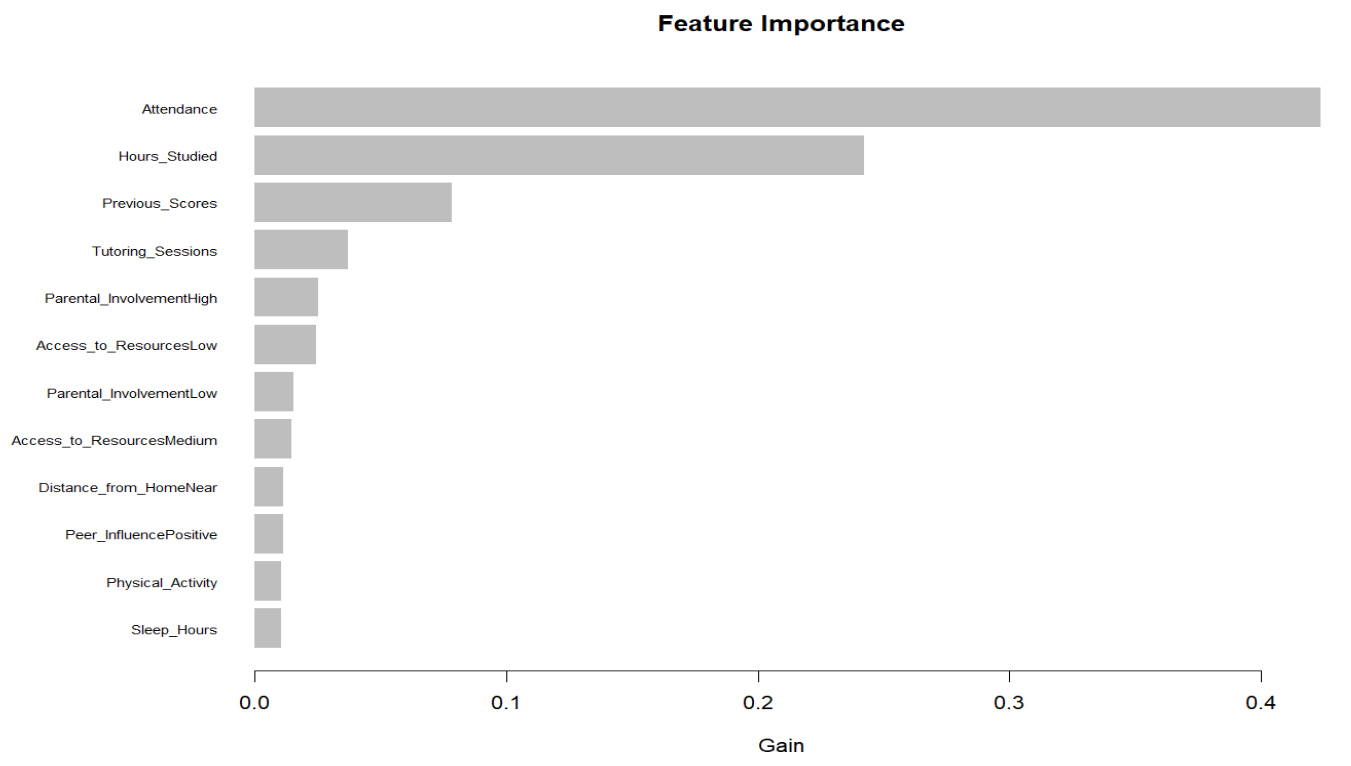
\includegraphics[width=0.8\textwidth,height=\textheight]{gbm_visual2.png}
\end{block}
\end{frame}



\end{document}
